% IMPORT SETTINGS
% OR START DOCUMENT WITH %&preamble TO USE THE PRECOMPILED PREAMBLE
\documentclass[english, 12pt]{article}
%! TEX root = /home/simon/Documents/artikel/main.tex


%%%%%%%%%%% LANGUAGE %%%%%%%%%%%

% For correct hyphenation in swedish
\usepackage[T1]{fontenc}

% For interpreting non-ASCII characters
\usepackage[utf8]{inputenc}

% International language support
% Fetches language from documentclass options. Most other packages do this as well
\usepackage{babel}


%%%%%%%%%%% FORMAL STUFF %%%%%%%%%%%

% Page margin lengths
\usepackage[top=3cm, bottom=3cm, inner=3cm, outer=3cm]{geometry}

% Dates & time
\usepackage[yyyymmdd]{datetime} % Useful when referencing websites
\renewcommand{\dateseparator}{-} % ISO 8601 date format

% Lists
\usepackage{enumerate} % Determines the style in which the counter is printed
\usepackage{enumitem} % Provides user control over the layout of the three basic list environments

% Citing & bibliography
\usepackage{csquotes} % For \enquote command for proper quotation marks, also biblatex recommends this
\usepackage[numbers]{natbib}


%%%%%%%%%%% PHYSICS %%%%%%%%%%%

\usepackage{braket} % Defines \bra, \ket, \braket, and \set
\usepackage{tensor} % Covariant index notation
\usepackage{physics} 

% Figure and table captions etc
\usepackage[font=small]{caption}


%%%%%%%%%%% MATHEMATICS %%%%%%%%%%%

% AMS packages
\usepackage{amsmath}
\usepackage{amsfonts}
\usepackage{amsthm}
\usepackage{amssymb}
\usepackage{mathrsfs}


%%%%%%%%%%% MISCELLANEOUS %%%%%%%%%%%

% This is a uglier but faster alternative to the todonotes package
\usepackage{xstring}
\usepackage[]{marginnote} 
\newcommand{\todo}[2][]{%
	\IfStrEqCase{#1}{%
        {inline}{{\color{red}#2}}%
	}[%
		\marginnote{\color{red}#2}%
	]
}

% Clickable links and refs
\usepackage{hyperref}								
\hypersetup{final, colorlinks, citecolor=black, filecolor=black, linkcolor=black, urlcolor=black}

% Cleverref automatically detects if you are referencing a figure, table, or equation etc
% Cleverref has to be loaded last I think, after babel and hyperref etc
\usepackage[noabbrev, nameinlink]{cleveref}
\crefname{equation}{}{}
\iflanguage{swedish}{ % Tell cleverref to use Oxford comma
	\newcommand{\creflastconjunction}{, och\nobreakspace}
}{}
\iflanguage{english}{
	\newcommand{\creflastconjunction}{, and\nobreakspace}
}{}

% Theorem and proof environments
% Has to be put after cleveref
\iflanguage{english}{
    \newtheorem{theorem}{Theorem}
    \newtheorem*{theorem*}{Theorem}
    \newtheorem{proposition}[theorem]{Proposition}
    \newtheorem*{proposition*}{Proposition}
    \newtheorem{corollary}{Corollary}[theorem]
    \newtheorem{corollary*}{Corollary}
    \newtheorem{lemma}[theorem]{Lemma}
    \newtheorem*{lemma*}{Lemma}
    \newtheorem{remark}[theorem]{Remark}
    \newtheorem*{remark*}{Remark}
    \theoremstyle{definition}
    \newtheorem{definition}[theorem]{Definition}
    \newtheorem*{definition*}{Definition}
    \newtheorem{axiom}[theorem]{Axiom}
    \newtheorem*{axiom*}{Axiom}
}{}

% Write \overset{text}&{=} in align environments to align with respect to the = symbol
\usepackage{aligned-overset} 

\usepackage[]{pifont} 
 
%! TEX root = /home/simon/Documents/artikel/main.tex

% Main number systems
\def\naturals{\mathbb{N}}
\def\integers{\mathbb{Z}}
\def\rationals{\mathbb{Q}}
\def\reals{\mathbb{R}}
\def\complexnumbers{\mathbb{C}}

% Some shorthands for correct spacing in math environments
\def\from{\colon} % Proper spacing of colon in f:A -> B
\newlength\mylen
\settowidth\mylen{$\longleftrightarrow$}
\newcommand*{\mapsbetween}{\longleftrightarrow\kern - 0.5\mylen\vline height 1.2ex depth -0.0pt\kern0.5\mylen} % Isomorphic \mapsto
\def\suchthat{\qq{s.th.}}
\def\definedas{\coloneqq}
\def\defines{\eqqcolon}
\newcommand*{\conjugate}[1]{\mkern 1.0mu\overline{\mkern-1.0mu#1\mkern-1.0mu}\mkern 1.0mu} % Complex conjugate
\newcommand*{\dual}[1]{{#1}^{*}} % Dual vector space
\newcommand*\ddual[1]{{#1}^{**}}

% Lie-groups & algebras, e.g. SU(n)
\newcommand*{\algebra}[2]{{\mathfrak{\MakeLowercase{#1}}}{\left(#2\right)}}
\newcommand*{\group}[2]{{\mathrm{\MakeUppercase{#1}}}{\left(#2\right)}}
% \newcommand*{\commutator}[2]{\left[#1, #2\right]}

% Fundamental operators
\def\sDiv{\mathscr{D}}
\def\sTwist{\mathscr{T}}
\def\sCurl{\mathscr{C}}
\def\sCurlDagger{\mathscr{C}^\dagger}

% Symmetric multiplication
\newcommand*{\SymMult}[2]{\overset{#1, #2}{\odot}}

% SymH
\DeclareMathOperator*{\Sym}{Sym}

% Notation for irreducible parts of symmetry operator coefficients
\newcommand*{\coeff}[3]{\underset{#2, #3}{#1}{}}

 
% \hypersetup{final} % Avoid warning about draft mode

\title{What is a tensor?\\Tensors from physics explained in unnecessary rigour using concepts from functional programming\\\ding{166}}
\author{Simon Jacobsson}
\date{\today}

\begin{document} 
\maketitle

If you ask a physics professor what a tensor is, they will likely tell you that \enquote{it is something that transforms like a tensor.}
I was personally a bit disappointed hearing this as a Master's student in theoretical physics, not only because of the apparent circularity of that statement, but because there was no interest in exploring the deeper mathematical reasons for why tensors kept appearing everywhere.
But those reasons \emph{are} interesting, and there \emph{is} a more insightful definition of tensors!
% Why is everything from cross products to moment of inertia described by tensors?

\section{Who is this explanation for?}%
\label{sec:who_is_this_explanation_for_}

This text is my attempt to write down what I wish I had been taught at the beginning of my Master's programme.
The explanation I am about to give is aimed at those with some university level maths and maybe physics also.
Ideally you have
\begin{itemize}
	\item heard of tensors before.
	Possibly in the context of physics, where you'll likely have seen Einstein's summation convention.
	\item had some linear algebra courses.
	You are comfortable with cross and dot products.
	It is good if you know what a linear space is.
	\item at some point programmed using some programming language.
\end{itemize}

If you google \enquote{what is a tensor}, there are already many people who have tried in many ways to answer this question.
Many of them also have strong opinions about the subject.
So please don't think of this as \emph{the} definition of tensors, but rather one of many ways to define them, which if nothing else shows off some cool ideas from programming.

\href{https://www.quora.com/Why-is-it-difficult-to-explain-tensors?}{\color{blue}This} question on Quora gives a fairly good overview over how difficutl tensors are to pin down.

\section{Linearity}%
\label{sec:linearity}

You can skip this section if you know what a linear space is.

Even though most of these definitions are completely general, let's for the sake of simplicity assume every linear space that we deal with is finite-dimensional.

Many physical equations are linear.
I don't know why exactly---if it is fundamental to nature somehow or if it's something we as humans impose on it because it's much easier to deal with.
If an equation isn't linear, we often go to great lengths to construct expansions of linear approximations.
I will take it as given that linearity is fundamental in some way.
\begin{axiom}\label{ax:linearity}
	Linearity is interesting.
\end{axiom}
\Cref{ax:linearity} entails both linear spaces and linear maps.
If you've only had one course in linear algebra, the former is probably a bit esoteric.
But a linear space is basically a set that you do linear transformations on.
So let's define things in that order.
\begin{definition}\label{def:linear_map}
	Let \(R\) be a field (\(\reals\) and \(\complexnumbers\) are examples of fields).
	If \(U\) and \(V\) are linear spaces over \(R\) and \(f \from U \to V\), then \(f\) is \emph{linear} if
	\begin{enumerate}
		\item $f(u + u') = f(u) + f(u')$ for all \(u\), \(u' \in U\).%
		\label{item:linearity_plus}
		\item \(f(c u) = c f(u)\) for all \(u \in U\) and all \(c \in R\).%
		\label{item:linearity_multiplication}
	\end{enumerate}
\end{definition}
This is pretty familiar stuff!
But if we think about it for a bit, what must be true about \(U\) for \cref{item:linearity_plus,item:linearity_multiplication} to make sense?
Well, if \(f\) maps from \(U\) and \(f(u + u')\) is well-defined, then \(u + u'\) should be in \(U\).
This should be true for all \(u\) and \(u'\).
Similarly, if \(f(c u)\) is well-defined, \(c u\) should be in \(U\) for all \(u \in U\) and all \(c \in R\).
We have some other things we generally want to be true about linear spaces, but this is basically it.
\begin{definition}\label{def:linear_space}
	Let \(R\) be a field.
	A set \(V\) is a \emph{linear space over \(R\)} if
	\begin{enumerate}
		\item For each \(u\), \(v \in V\), there is a unique element \(u + v \in V\) (addition).
		\item For each \(u \in V\) and each \(c \in R\), there is a unique element \(c u\) (multiplication with scalar).
	\end{enumerate}
	and
	\begin{enumerate}
		\setcounter{enumi}{2}
		\item \(u + v = v + u\) for all \(u\), \(v \in V\).
		\item \((u + v) + w = u + (v + w)\) for all \(u\), \(v\), \(w \in V\).
		\item There is an element \(\mathit 0 \in V\) such that \(\mathit 0 + u = u + \mathit 0 = u\) for all \(u \in V\).
		\item For each \(u \in V\) there exists an element \(-u \in V\) such that \(u + (-u) = (-u) + u = \mathit 0\).
		\item \(a(b u) = (a b) u\) for all \(a\), \(b \in R\) and all \(u \in V\).
		\item \(a (u + v) + (a u) + (a v)\) for all \(a \in R\) and all \(u\), \(v \in V\).
		\item \((a + b) u = (a u) + (b u)\) for all \(a\), \(b \in R\) and all \(u \in V\).
		\item \(1 u = u\) for all \(u \in V\).
	\end{enumerate}
\end{definition}

As mentioned, this is just a list of formal requirements that sets must satisfy for it to make sense to apply linear functions to their elements.
These particular kinds of requirements lists are known in functional programming as \emph{typeclasses}.
A simpler example of a typeclass is \emph{totally ordered sets}, which are sets \(S\) with a some binary operation \(\leq \from S \times S \to \set{\textrm{True}, \textrm{False}}\) satisfying
\begin{enumerate}
	\item \(x \leq x\).
	\item \(x \leq y\) and \(y \leq x\) \(\implies x = y\).
	\item \(x \leq y\) and \(y \leq z\) \(\implies x \leq z\).
	\item Either \(x \leq y\) or \(y \leq x\).
\end{enumerate}
For all \(x\), \(y\), \(z\) \(\in S\).

Note that, in \cref{item:linearity_plus,item:linearity_multiplication} of \cref{def:linear_map}, the addition and multiplication with scalar are different operators on each side of the equals sign.
In the left-hand side of \cref{item:linearity_plus}, \(+ \from U \times U \to U\), while in the right-hand side \(+ \from V \times V \to V\).
Both of these operators should of course satisfy \cref{def:linear_space} for \(U\) and \(V\) respectively.

Let's also define what we mean when we say that two linear spaces are equal.
\begin{definition}
	Two linear spaces \(U\) and \(V\) over a field \(R\) are \emph{isomorphic} if there exists some linear bijection \(f \from U \to V\).
	\(f\) is then an \emph{isomorphism}.
\end{definition}

Two examples of linear spaces are \(\reals^2\) over \(\reals\) and \(\complexnumbers\) over \(\reals\).
These two are in fact isomorphic, easily seen by extending the map \((1, 0) \mapsto 1\), \((0, 1) \mapsto i\) linearly.
Another example which is not isomorphic to those two is \(\complexnumbers\) over \(\complexnumbers\), which shows the importance of having the field in mind.

A useful notion in linear algebra is the dual space.
\begin{definition}\label{def:dual_space}
	Let \(V\) be a linear space over \(R\).
	The \emph{dual space} \(\dual V\) to \(V\) is the set of linear maps \(\from V \to R\).
\end{definition}

If \(\langle \cdot, \cdot \rangle\) is the natural inner product on \(\reals^n\), then an example of a dual space is
\begin{align*}
	\dual{(\reals^n)} = \set{ \langle v, \cdot \rangle \quad \textrm{s.th.} \quad v \in \reals^n}.
\end{align*}

\begin{proposition}\label{prop:dual_dual_space}
	\(\ddual V = V\).
\end{proposition}

You can prove this if you want to, but, for me at least, it feels like it really should be true.


\section{Einstein's summation convention}%
\label{sec:einstein_s_summation_convention}

Index notation, primarily used in relativistic physics, builds on Einstein's summation convention.
Allegedly, this was one of the discoveries that Einstein was most thrilled about: that when writing out the components in linear algebraic expressions, repeated indices are always summed over.
So if \(v \in V\) is a vector with components \(v_\alpha\) in an orthonormal basis \(B\) and \(L \from V \to V\) is a linear map with components \(L{}^\alpha{}_\beta\) in \(B\), then \(L(v)\) has components
\begin{align*}
	\sum_\alpha L{}^\alpha{}_\beta v_\alpha,
\end{align*}
or, with Einstein's summation convention,
\begin{align*}
	L{}^\alpha{}_\beta v_\alpha.
\end{align*}

In this text, I will use something similar but different: \emph{abstract indices}.
In abstract index notation, indices no longer denote components but the actual tensors themselves.
If \(v_a \in V\) is a vector and \(L{}^a{}_b \from V \to V\) is a linear map, then the action of \(L{}^a{}_b\) on \(v_a\) is still written
\begin{align*}
	L{}^a{}_b v_a,
\end{align*}
but the repeated index does not mean summation anymore.
It just means \emph{action}.

In this context, a repeated index is called a \emph{contraction}.


\section{Partial application}%
\label{sec:partial_application}

In the more well-known programming languages like Java, Python, C, etc., the usual procedure is to define some variables and then modify those until you get them to the state that you want them to be in.
Consider for example the short Python program below and its output,
\begin{verbatim}
L = [1, 4, 3, 2]
L.sort()
print(L)

out: [1, 2, 3, 4]
\end{verbatim}
Note that using the method \verb|sort()| changes the state of \verb|L|.

In contrast, with functional programming like Haskell, you can't modify variables once they're defined.
All you can do is to write down all of the variables you want to use and then apply functions to them.
I use the word \enquote{function} here in its strict mathematical sense: A \emph{function} (or \emph{map}) \(f\) from a set \(A\) to a set \(B\) is a rule that assigns, to each \(a \in A\), a unique \(b \in B\).
We often write \(f \from a \mapsto b\) or \(f(a) = b\).
Importantly, this means that
\begin{enumerate}
	\item a function does alter any state---there's no function for switching your clock from winter time to summer time.
	\item for a given argument \(a\), a function \emph{always} returns the same element \(b\).
\end{enumerate}

It may seem that this is very limiting, but it actually turns out that writing code this way feels much more like doing maths than the other type of coding!
Since everything that you can use are functions, you get very intimate with the properties of functions when programming functionally.

One important concept is \emph{partial application}, or \emph{currying}.
Consider a function \(f\) that takes two arguments.
Maybe it looks like this: \(f \from A \times B \to C\).
What if you know that the first argument you'll be supplying is \(a \in A\)?
Then for all intents and purposes, you have a new function \(g \from B \to C\) defined by \(g(b) = f(a, b)\).
But you will also have a different such function for each \(a\).
So you can think of \(f\) really as a function \(\hat f\from A \to B^C\) where \(B^C\) denotes the set of functions from \(B\) to \(C\).

Are \(f\) and \(\hat f\) really so different then?
In many cases, I would like to be agnostic about the amount of arguments that I'm about to supply for \(f\).
In functional programming, \(f\) and \(\hat f\) are the same object!
It is written
\begin{align*}
	f \from A \to B \to C.
\end{align*}
The function \(\hat f \from a \mapsto g\) is called a partial application of \(f\) to \(a\).

As an example, consider the following Haskell program,
\begin{verbatim}
bool2Int True = 1
bool2Int False = 0
heaviside = bool2Int . ( > 0)
\end{verbatim}
which defines the Heaviside step function
\begin{align*}
	H(x) =
	\begin{cases}
		0, \quad x < 0\\
		1, \quad x > 0
	\end{cases}.
\end{align*}
Writing \verb|( > 0)| means we partially apply the comparison \verb|<|\(\from \reals \times \reals \to \set{\textrm{True}, \textrm{False}}\) to \(0\).
The dot on the third line just means \emph{composition}, we compose the function \verb|( > 0)| \(\from \reals \to \set{\textrm{True}, \textrm{False}}\) with \verb|bool2Int|\(\from \set{\textrm{True}, \textrm{False}} \to \reals\).


\section{Defining tensors as multilinear maps}%
\label{sec:defining_tensors_as_multilinear_maps}

A \emph{multilinear map} is a function that takes several arguments and is linear in each one.
Cross products are an example since
\begin{align*}
	(\vec{a} + \vec{b}) \times \vec{c} ={}& \vec{a} \times \vec{c} + \vec{b} \times \vec{c},\\
	(r \vec{a}) \times \vec{b} ={}& r (\vec{a} \times \vec{b}),\\
	\vec{a} \times (\vec{b} + \vec{c}) ={}& \vec{a} \times \vec{b} + \vec{a} \times \vec{c},\\
	\vec{a} \times (r \vec{b}) ={}& r (\vec{a} \times \vec{b}).
\end{align*}
Another example is scalar products for similar reasons.
Yet another example is the (signed) volume of a parallelepiped.
If you have three vectors \(\vec a\), \(\vec b\), and \(\vec c\) in \(\reals^3\), then they define a parallelepiped by \cref{fig:parallelepiped}.
Look closely at the figure and try to see why each vector contributes linearly to the volume.

\begin{figure}[ht]
	\centering
	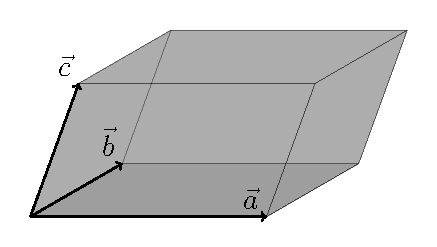
\includegraphics[]{figures/parallelepiped.pdf}
	\caption{If \(\vec a\), \(\vec b\), and \(\vec c\) are positively oriented according to the right-hand rule, then the volume is positive.}%
	\label{fig:parallelepiped}
\end{figure}

The magic is admittedly a bit lost if you know that the signed volume of the parallelepiped is \(\vec a \cdot (\vec b \times \vec c)\).
But there \emph{are} examples of multilinear maps that are not cross or dot products.
The \emph{outer product} of two vectors is
\begin{align}\label{eq:outer_product}
	(
	\begin{bmatrix}
		u_1\\
		u_2\\
		u_3
	\end{bmatrix},
	\begin{bmatrix}
		v_1\\
		v_2\\
		v_3
	\end{bmatrix}
	)
	\mapsto
	\begin{bmatrix}
		u_1\\
		u_2\\
		u_3
	\end{bmatrix}
	\begin{bmatrix}
		v_1&
		v_2&
		v_3
	\end{bmatrix}
	=
	\begin{bmatrix}
		u_1 v_1 & u_1 v_2 & u_1 v_3\\
		u_2 v_1 & u_2 v_2 & u_2 v_3\\
		u_3 v_1 & u_3 v_2 & u_3 v_3\\
	\end{bmatrix}.
\end{align}

So these are a few examples of multilinear maps.
Now let's make the definition that you came here to for.
\begin{definition}\label{def:tensor}
	Let \(V\) be a linear space over a field \(R\).
	A valence \((k, l)\) \emph{tensor} is multilinear map
	\begin{align*}
		f \from \underbrace{V \times \dots \times V}_{\times l} \to \underbrace{V \times \dots \times V}_{\times k}.
	\end{align*}
	Or, equivalently, a tensor is a multilinear map
	\begin{align*}
		f \from \underbrace{V \times \dots \times V}_{\times l} \times \dual V \to \underbrace{V \times \dots \times V}_{\times (k - 1)}
	\end{align*}
	or a multilinear map
	\begin{align*}
		f \from \underbrace{V \times \dots \times V}_{\times (l - 1)} \to \dual V \times \underbrace{V \times \dots \times V}_{\times k}
	\end{align*}
	etc.
\end{definition}
To see the isomorphism between these sets of multilinear maps, we will use partial application, along with \cref{prop:dual_dual_space}.
For the special case of a map \(f \from V \to V\), the argument goes like this.
Map \(f \from V \to V\) to the multilinear \(f' \from V \times \dual V \to R\) by \(f'(v, \dual u) = \dual u(f(v))\).
Then map \(f' \from V \times \dual V \to R\) to \(f'' \from V \to \dual{(\dual V)}\) by \(f''(v) = f'(v, \cdot)\).
But since \(\dual{(\dual V)} = V\), \(f'' \from V \to V\).
The kernels of each of the two maps \(f \mapsto f'\) and \(f' \mapsto f''\) are clearly \(0\) and they are both clearly linear, so each of them must be an isomorphism%
\footnote{%
There are three statements here that must be motivated: \(\operatorname{ker}(f \mapsto f') = 0\), \(\operatorname{ker}(f' \mapsto f'') = 0\), and that \(f \mapsto f''\) is an isomorphism.
Can you come up with concise arguments for these when \(V\) is infinite-dimensional?
I don't think that I can.
}.
It is not hard to extend this argument to all different kinds of combinations of \(V\) and \(\dual V\).

The preceding paragraph is fairly dense and contains some plausible-sounding but non-obvious things.
Read it slowly.
In essence, it proves that we can write tensors as multilinear maps
\begin{align*}
	f \from \underbrace{V \to \dots \to V}_{\times l} \to \underbrace{\dual V \to \dots \to \dual V}_{\times k} \to R.
\end{align*}


\section{Contractions}%
\label{sec:contractions}

With index notation, we can consicely show the valence of a tensor.
$f \from V \to V \to \dual V \to \dual V \to \dual V \to R$ may profitably be written as $f{}_{a b}{}^{c d e}$.
But writing indices in this way also helps us denote partial applications in a way that uniquely tells us \emph{which} partial applications are made.

Here's the bridge between tensors as multilinear maps and tensors as indexed objects: contractions are partial applications.
As an example, consider a valence $(2, 1)$ tensor
\begin{align*}
	X{}_a{}_b{}^c \from V \to V \to \dual V \to R
\end{align*}
and a valence $(0, 2)$ tensor
\begin{align*}
	Y{}^{}a{}^b \from \dual V \to \dual V \to R.
\end{align*}
Now, one way of viewing these tensors is to view $X{}_a{}_b{}^c$ as a map $\from V \times V \to V$ and $Y{}^a{}^b$ as an element in $V \times V$.
Then we can of course act on $Y{}^a{}^b$ with $X{}_a{}_b{}^c$,
which is written
\begin{align*}
	X{}_a{}_b{}^c Y{}^a{}^b
\end{align*}
and yields a valence $(1, 0)$ tensor (vector in $V$).
But $X{}^a{}_b{}_c$ can also be seen as a map $\from V \to V^V$.
Then, applying $X{}^a{}_b{}_c\from V \to V^V$ to the first part of $Y{}^a{}^b$, written
\begin{align*}
	X{}^a{}_b{}_c Y{}^c{}^d,
\end{align*}
yields a valence $(2, 1)$ tensor.

The relation between this definition of contraction and the \enquote{repeated indices are summed over}-one is that they're the same thing if we do contraction explicitly in an orthogonal basis for $V$.
Remember that in my notation $X{}^a{}_b{}_c$ \emph{is} the tensor while in regular index notation $X{}^a{}_b{}_c$ is its components in some given basis.
So now is a pretty good time to reflect a bit on what we have actually done.
For I didn't need to mention any basis until this paragraph, so everything we have done thus far is totally basis-independent!

\section{Tensor product}%
\label{sec:tensor_product}

You could stop reading here and still get away with a pretty solid understanding of what a tensor is, but if you're interested, we could talk a bit about the symbol \(\otimes\) that you may have seen in relation to tensors.

\begin{definition}\label{def:tensor_product}
	Let \(U_1\), \dots, \(U_n\) be vector spaces over a field \(R\).
	Then \(U_1 \otimes \dots \otimes U_n\) is a linear space equipped with a multilinear map \(\pi \from U_1 \times \dots \times U_n \to U_1 \otimes \dots \otimes U_n\) such that for any multilinear map \(f \from U_1 \times \dots \times U_n \to R\) there exists a unique linear map \(g \from U_1 \otimes \dots \otimes U_n \to R\) such that \(f = g \circ \pi\).
\end{definition}

The space \(U \otimes V\) is called the \emph{tensor product space} of \(U\) and \(V\).
\Cref{def:tensor_product} is fairly dense, but what it says is basically that for every function bilinear on \(U \times V\), there is a function that is linear on \(U \otimes V\).
So we have yet another way of writing \cref{def:tensor}: a tensor is a linear map
\begin{align*}
	f \from \underbrace{V \otimes \dots \otimes V}_{\times l} \otimes \underbrace{\dual V \otimes \dots \otimes \dual V}_{\times k} \to R.
\end{align*}

This looks somewhat familiar thought.
Recalling \cref{def:dual_space}, we can rewrite the set of valence \((k, l)\) tensors as
\begin{align*}
	&\set{f \quad \textrm{s.th.} \quad f \textrm{ is a valence \((k, l)\) tensor}}\\
	%
	={}& \set{f \from \underbrace{V \otimes \dots \otimes V}_{\times l} \otimes \underbrace{\dual V \otimes \dots \otimes \dual V}_{\times k} \to R \quad \textrm{s.th.} \quad f \text{ is linear}}\\
	%
	={}& \dual{\big( \underbrace{V \otimes \dots \otimes V}_{\times l} \otimes \underbrace{\dual V \otimes \dots \otimes \dual V}_{\times k} \big)}\\
	%
	={}& \underbrace{\dual{V} \otimes \dots \otimes \dual{V}}_{\times l} \otimes \underbrace{V \otimes \dots \otimes V}_{\times k}.
\end{align*}
The last step is that taking the dual space distributes over tensor products.
It is not hard to believe, and it is not difficult to prove%
\footnote{%
	The idea is that \(\phi \from \dual V \otimes \dual W \to \dual{(V \otimes W)}\) defined by \(\phi(f \otimes g)(v \otimes w) = f(v) g(w)\) is an isomorphism.
}.
Hence we can make one last very neat reformulation of \cref{def:tensor}: A tensor is an element of
\begin{align*}
	\underbrace{\dual{V} \otimes \dots \otimes \dual{V}}_{\times l} \otimes \underbrace{V \otimes \dots \otimes V}_{\times k}.
\end{align*}


\section{Krönecker product}%
\label{sec:krönecker_product}

This is all very elegant, but it is at the same time very abstract, and it would be useful to see how these concepts look in the wild.
Enter the Krönecker product, which is \emph{a} tensor product.
You can use it for finite-dimensional spaces for which you have a basis.
\begin{definition}
	Let
	\begin{align*}
		A =
		\begin{bmatrix}
			A_{11} & \dots & A_{1n}\\
			\vdots & \ddots & \vdots\\
			A_{m1} & \dots & A_{mn}
		\end{bmatrix}
	\end{align*}
	and
	\begin{align*}
		B =
		\begin{bmatrix}
			B_{11} & \dots & B_{1q}\\
			\vdots & \ddots & \vdots\\
			B_{p1} & \dots & B_{pq}
		\end{bmatrix}
	\end{align*}
	be two matrices with entries in a field $R$.
	The \emph{Krönecker product} of $A$ and $B$ is
	\begin{align*}
		\pi(A, B) =
		\begin{bmatrix}
			A_{11}
			\begin{bmatrix}
				B_{11} & \dots & B_{1q}\\
				\vdots & \ddots & \vdots\\
				B_{p1} & \dots & B_{pq}
			\end{bmatrix}
			& \dots &
			A_{1n}
			\begin{bmatrix}
				B_{11} & \dots & B_{1q}\\
				\vdots & \ddots & \vdots\\
				B_{p1} & \dots & B_{pq}
			\end{bmatrix}\\
			%
			\vdots & \ddots & \vdots\\
			%
			A_{m1}
			\begin{bmatrix}
				B_{11} & \dots & B_{1q}\\
				\vdots & \ddots & \vdots\\
				B_{p1} & \dots & B_{pq}
			\end{bmatrix}
			& \dots &
			A_{mn}
			\begin{bmatrix}
				B_{11} & \dots & B_{1q}\\
				\vdots & \ddots & \vdots\\
				B_{p1} & \dots & B_{pq}
			\end{bmatrix}
		\end{bmatrix}.
	\end{align*}
	So $\pi(A, B)$ is a $mp \times mq$ matrix and an is element of the tensor product space $R^{mn} \otimes R^{pq}$.
	$\pi(A, B)$ is denoted $A \otimes B$.
\end{definition}

The tensor product space $R^{mn} \otimes R^{pq} = R^{mp \times mq}$ is much larger than the Cartesian product space $R^{(m + p) \times (n + q)}$, which reflects the fact that it less restrictive to be multilinear than to be linear.

We had an example earlier, \cref{eq:outer_product}, of a multilinear map.
We can see now that this is just $\vec u \otimes \vec v$.
Hence, for each bilinear function that $f$ takes two real $3$-vectors, there is a linear function $g$ that takes one real $3\times3$-matrix such that $f(\vec u, \vec v) = g(\vec u \otimes \vec v)$.

\section{How to transform like a tensor}%
\label{sec:how_to_transform_like_a_tensor}

What about the physics professor's definition of a tensor?
Well, let's think about what happens to the components of a tensor \(T{}_i{}^j \from V \to \dual V \to R\) when we make a coordinate change to \(V\).
If \(v\) is a vector in \(V\) whose components transform as \(v{}^i \mapsto A{}_j{}^i v{}^j\) by a change of coordinates, and if \(\dual v = \langle v, \cdot \rangle \in \dual V\), then the components of \(\dual v\) should transform as \((\dual v)_i \mapsto (A^{-1}){}^j{}_i (\dual v){}_j\).
The reason for this is that \(|v|^2 = \dual v v\) is invariant under coordinate changes, and
\begin{align*}
	\dual v v ={}& v{}^i (\dual v){}_i\\
	\mapsto{}& v{}^j A{}_j{}^i (A^{-1}){}^k{}_i (\dual v){}_k\\
	={}& v{}^j \delta{}_j{}^k (\dual v){}_k\\
	={}& \dual v v
\end{align*}
shows that this is satisfied.
So with some abuse of notation, let's write down how \(T(v, \dual v)\) transforms:
\begin{align*}
	T{}_i{}^j\big(
		v{}^i,
		(\dual v){}_j
	\big)
	\mapsto{}& T\big(
		A{}_k{}^i v{}^k,
		(A^{-1}){}^l{}_j (\dual v){}_l
	\big)\\
	%
	={}& A{}_k{}^i (A^{-1}){}^l{}_j T{}_i{}^j
	\big(
		v{}^k,
		(\dual v){}_l
	\big).
\end{align*}
Hence the components of \(T{}_i{}^j\) transform as
\begin{align}\label{eq:tensor_transformation_rules}
	T{}_i{}^j \mapsto A{}_k{}^i (A^{-1}){}^l{}_j T{}_i{}^j.
\end{align}

In physics you often deal with tensor fields.
Now I don't use \enquote{field} as in \(\reals\) or \(\complexnumbers\) anymore but as in a function from the space or spacetime manifold \(M\) to the space of tensors.
Then \(V\) is often the tangent space to \(M\).
If we make a coordinate change \(x \mapsto \hat x\) on \(M\), then that induces a coordinate change \(A{}_i{}^j = \partial \hat x_i / \partial x_j\) of the tangent space.
But just substituting this into \cref{eq:tensor_transformation_rules} and using \(\left(\partial \hat x_i / \partial x_j\right)^{-1} = \partial x_i / \partial \hat x_j \) gives
\begin{align*}
	T{}_i{}^j \mapsto \frac{\partial \hat x_k}{\partial x_i} \frac{\partial x_j}{\partial \hat x_l} T{}_i{}^j.
\end{align*}
This is the transformation law that physicists mean when they say something transforms as a tensor.
It generalizes in the obvious way for higher valence tensors.


\end{document}
